\hypertarget{sec:dsac-discovery}{%
\chapter{Conversational-based Discovery \& Composition Assistant}\label{sec:dsac-discovery}}
Referring to the scenario in \cref{sec:scenario}, the importance of enhancing the tool’s expressive power through natural language-enabled interaction is highlighted. This chapter presents two mechanisms to address the issues related to “Poor expressive power” to achieve Objective \cref{ro:1}. The Discovery Chatbot supports domain experts during the component discovery phase by providing a natural language-based interaction medium. The Solution Designer choreographs the selected components by identifying the compatibility paths among them. This will be later integrated into the composition model as the communication configuration. An evaluation process is conducted to assess these tools’ performance.


\hypertarget{sec:disc.analysis}{%
\section{Analysis}\label{sec:disc.analysis}}
\vspace{10pt}
Due to the rapid increase in quantity and complexity of web \gls{api}s, the discovery process has become an important challenge from the end-user’s perspective \autocite{Fariss2018}. Furthermore, the composition’s expressiveness depends heavily on the number of solution classes that it can propose and how closely they align with the domain expert’s intentions. In such cases, developing an automated and scalable discovery mechanism is crucial for ensuring the composite application’s  efficiency \autocite{Zarei2020}. 

According to the study conducted in \autocite{Ponce2022}, current \gls{eud} tools struggle to find the right balance between usability for domain experts and increased expressive power for complex use-case scenarios. Since maximum expressiveness can make the tool too complex for the domain expert, the goal in this chapter is to minimize the gap between the domain expert’s intentions and the result tool. During the next section, we review state-of-the-art service discovery methods. \cref{sec:discovery-module} presents an overview of the discovery module, which comprises two primary components: \gls{disco}, responsible for identifying the most suitable components, and the Solution Designer, which generates the compatibility graph to be integrated with composition model by Composition Engine (cf. \cref{sec:dsac-composer}). These tools are discussed in detail in \cref{sec:disco} and \cref{sec:solution-Designer}, respectively. At the end of this chapter, the evaluation process is presented in \cref{sec:disco-evaluation}.


\vspace{-10pt}
\hypertarget{sec:discovery.related-work}{%
\section{Related Work}\label{sec:dsac-disco.related-work}}
\vspace{10pt}

Verity of solutions have been proposed for component discovery in service composition applications. Solutions can be categorized considering various factors such as application requirements or \gls{qos}. According to \autocite{Tschudnowsky2016} two solution classes are bottom- up composition engines, in which the higher goal is not taken into the account and top-down application compositions where the starting point is the description of the user’s higher goal. Our discovery approach falls into the top-down composition solutions.

In this work we focused on the semantic-based technique due to its relevance to our defined requirements. Semantic-based solutions are retrieving the semantically similar components based on the user’s goals. Logic-based and non-logic-based approaches are the two main categories of semantic-based solutions \autocite{Jalali2014}. The logic-based approaches performing logical reasoning on the user’s query using proper domain ontology. While in non-logic-based approaches the discovery is performed by measuring the text similarity among the service description and user’s query. Logic-based approaches, on the other hand, allowing the automatic discovery  to guarantee finding the best-fitting domain specific components \autocite{Zhang2018}. 


\vspace{-10pt}
\hypertarget{sec:discovery-module}{%
\section{Discovery and Composition Module}\label{sec:discovery-module}}
\vspace{10pt}

The goal of the discovery module is to discover the best-fitting components to be composed to answer the domain expert’s situational requirements. The \gls{bpmn} diagram in Figure 6.1 shows the discovery and composition solution generation. This process is implemented by the \gls{disco}, that provides a domain-specific conversational interface (aka chatbot) capable of finding the best-fitting components. \gls{disco} expands the domain expert’s queries, by leveraging the query expansion techniques, to identify the target domain and operations needed to achieve the final result.

\begin{figure}[hbt]
\hypertarget{fig:discovery-process}{%
\centering
\includegraphics[width=0.85\textwidth]{../figures/MyFigures/d&C (1).drawio.pdf}
\captionsetup{justification=centering}
\caption{Discovery Process}\label{fig:discovery-process}
}
\end{figure}

According to the \cref{fig:discovery-process}, the domain expert communicates with the
\gls{disco} using a dialogue-based interface. Upon receiving an utterance, the
\emph{\gls{nl} Unit} produces the query parameters and send them to the
\emph{Component Retrieval Engine} which retrieves the best-fitting
components from the component repository. The \emph{Solution Designer}
utilizes this data to construct the \emph{Compatibility graph}, which
presents the optimum orchestration of the components according to the
identified goals. This graph is then integrated into the Composition
Model by the Composition Engine detailed in the \cref{sec:composition-imp}.

\vspace{-10pt}
\hypertarget{sec:disco}{%
\section{\gls{disco}}\label{sec:disco}}
\vspace{10pt}

Conversational interfaces, also known as chatbots, provide a popular
medium for interaction between users and smart devices as well as web
services. Leveraging chatbot technology and conversational interfaces,
such as Siri, Amazon Alexa, and Google Assistant, demonstrates promising
results in enhancing usability and expressiveness in both industry and
academic domains \autocite{Raghuvanshi2018}. Chatbots generate realistic
responses to users' queries by mimicking human intelligence. According to 
research by \autocite{Fuckner2013}, using natural language-enabled interfaces 
increases efficiency by 30\% in terms of time and 60\% in terms of effort. 
Moreover, these interfaces improve retrieval accuracy by guiding users towards 
more informative interactions \autocite{Zarei2020}.

With this in mind, \gls{disco} is designed to assist domain experts with
component discovery. It engages in bi-directional conversations with
domain experts to gather key important parameters such as goals, desired
operations, and the target domain, to identify best-fitting components.
In each conversation round, \gls{disco} generates a reasonable response
according to the domain expert's input. This process results in a list 
of component candidates, which are then evaluated based on a rating scale 
to choose the final set. The design of \gls{disco} is guided by the following two principles:
\begin{itemize}
  \item
  The components are grouped according to their predefined domains. Depending on their relevance, a service can be assigned to multiple domains.
  \item
  This tool does not require domain experts to undergo the model training phase. Typically, chatbots require model training before use which is a time-consuming process. However, \gls{disco} automates this step, offering domain-specific models based on the textual data provided by domain experts.
  \end{itemize}

\gls{disco} employs a customized version of the input-intent-action-response
conversation model \autocite{Baez2020}. In the original model,
the user's intent is extracted from the input such as ``change the group
meeting from Wednesday, July 4th, to Tuesday'' with the help of the
Natural Language Understanding (NLU) unit. The intent (e.g., "change
the group meeting entry in the calendar"), is then mapped to a set of
corresponding actions to realize the user's goal ("addToCalander").
Based on the action's result, a suitable response is generated (e.g.,"
Your meeting has been successfully changed to Tuesday''). To tailor this
conversation model to the situational needs of domain experts,
the~I\emph{ntent} and~A\emph{ction} phases are refined. In the Intent
phase, key parameters such as the target domain and desired operations
are identified. These parameters are essential for retrieving the
suitable components aligned with domain expert\textquotesingle s goals
\autocite{Zhang2020}. The action phase is then referred to as the
matchmaking process to retrieve the most relevant components.

\begin{figure}[hbt]
\hypertarget{fig:disco-arch}{%
\centering
\includegraphics[width=0.85\textwidth]{../figures/MyFigures/Overview.drawio.pdf}
\captionsetup{justification=centering}
\caption{\gls{disco} Architecture Overview}\label{fig:disco-arch}
}
\end{figure}

\cref{fig:disco-arch} illustrates the overall architecture of \gls{disco}, which comprises two primary modules: Natural \gls{nlu} Language Understanding (NLU) and \gls{dm}.Together these modules referenced as NL Unit in \cref{fig:discovery-process}. These modules are reviewed in detail in the following two sections.


\vspace{-10pt}
\hypertarget{sec:nlu}{%
\subsection{Natural Language Understanding}\label{sec:nlu}}
\vspace{10pt}

\gls{nlu} analyzes the domain expert's input to extract parameters such as
target domain, operations, and entities. These parameters are used to
instantiate the \emph{Request Template} during runtime. The Request
Template, defined in \gls{xml} syntax, is a generic description that
summarizes the domain expert's intention. This template is later used
during the matchmaking process to retrieve components. The NLU consists
of three primary modules: the \gls{pu}, Classifiers, and
Dependency Parser. The \gls{pu} annotates the input with tokens and performs
the preprocessing steps such as stop words removal, and part-of-speech
tagging. The output is then used as the input for the Domain, and Entity
classifiers. Classifiers play an important role in chatbots by
normalizing the input queries and segmenting them into logical parts
\autocite{Abdul-Kader2015}.

\textbf{Domain Classifier} identifies the target domain based on the
input query. Identifying the domain enhances the discovery process by
limiting the search space to functionally similar component \autocite{Zhang2018}. To achieve this, representative words for each domain are
identified by applying the TF-IDF technique on domain-related textual
corpora. These representative words are those with the highest frequency
in the domain taxonomy, as approved by domain experts. To identify the
target domain, the Word2vec algorithm computes the similarity between
the core nouns in the input query and each domain's representative
words. This similarity is measured by cosine similarity between the
query's noun vector \(Q\) and domain's representative set, DR using the
following formula:

\begin{equation}
\cos\theta = \frac{Q \cdot DR}{||Q|| \, ||DR||}
\end{equation}

The domain classifier prioritizes the core nouns of a query due to their greater importance compared to verbs. For example, the queries: "buy flight tickets" and "buy a house" refer to different domains, as indicated by the core nouns "flight" and "house" \autocite{Zhang2018}. 

The following algorithm presents this procedure in detail.

\setlength{\algomargin}{2em} %
\begin{algorithm}
	\DontPrintSemicolon
	\KwIn{Pre-processed query \(q\), Vector representation of the
	domain representative word set \({rs}_{d}\)}
	\KwOut{The target domain}
	
	\begin{enumerate}
	\item 
	Extracts the core nouns \(\mathbf{q}_{\mathbf{n}}\) from the query
	  \(\mathbf{q}\)
	\item 
	Create the vector representation of the \(\mathbf{q}_{\mathbf{n}}\)
	\item 
	For each \(\mathbf{rs}_{\mathbf{d}}\) calculate the sim
	  (\(\mathbf{rs}_{\mathbf{d}}\mathbf{,\ }\mathbf{q}_{\mathbf{n}}\))
	\item 
	Return the \(\mathbf{rs}_{\mathbf{d}}\) with the highest similarity
	  value
	\end{enumerate}
	
\caption{Target Domain Identification}\label{alg:disc-domain}
\end{algorithm}


\textbf{Entity Classifier} identifies and labels real-world objects such
as locations, persons, countries, etc. These entities can serve as
parameters for components. For instance, in the sentence "find a Mark
Twain's book that costs \$30", the identifiers PERSON (Mark Twain) and
MONEY (\$30) are assigned.

The open-sourced library spaCy\footnote{\url{https://spacy.io/}} is used
for entity recognition. To train models, we used the
OntoNotes5\footnote{\url{https://catalog.ldc.upenn.edu/LDC2013T19s}}
corpus which includes various texts such as conversations and news
articles. This model is capable of identifying 18 different types of
entities.


\textbf{Dependency Parser}

The dependency parser plays a crucial role in retrieving the necessary
functionalities to accomplish given tasks. Each component offers
multiple functionalities, referred to as operations. Taking these
operations into account during the discovery phase can enhance precision
\autocite{Zarei2021}. In this context a component operation is
defined as \(cf = < AV,AN,\ \{ P_{i}\} >\) where \emph{AV} represents
the action verbs describing a component operation, \emph{AN} denotes the
action nouns affected by the operations. The set of component parameters
are denoted by \(P_{i}\). For instance, the query "Find hotels in
Berlin" can be formulated as \(sf\  = < find,hotels,\{ Berlin\} >\). An
empty output in this context is represented by ``\(-\)''.

To enhance the original query and capture a more comprehensive meaning,
the query expansion technique is used. This technique involves adding
relevant phrases and meaningful terms to the initial query. A Dependency
Parser extracts the grammatical dependencies among pairs of words.
Certain dependencies can reflect the requester\textquotesingle s
intended functionalities. In this work, we focused on four primary
dependencies: nominal subject (nsubj), direct object (dobj), indirect
object (iobj), and preposition (prep). According to the Universal
Dependencies\footnote{https://universaldependencies.org/} such
dependencies are considered core arguments in the English language.
Figure 6.3 demonstrates how the desired operations can be extracted from
the query, "\emph{A service to calculate the tax rate and insurance for
international products}" using query expansion.

\begin{figure}[hbt]
\hypertarget{fig:disco-query-exp}{%
\centering
\includegraphics[width=0.85\textwidth]{../figures/MyFigures/QE.pdf}
\captionsetup{justification=centering}
\caption{Query Expansion Process by Dependency Parser}\label{fig:disco-query-exp}
}
\end{figure}

The initial dependencies are extracted using the \gls{nltk} toolkit, selected for its superior precision relative to alternative parsers \autocite{Zhang2019}. Through a detailed analysis of these initial dependencies and careful consideration of the grammatical function of each typed dependency within a sentence, The Algorithm 6.2 to extract component operations based on the query's grammatical information.

\setlength{\algomargin}{2em} %
\begin{algorithm}
	\DontPrintSemicolon
	\KwIn{Pre-processed query \(q\)}
	\KwOut{List of desired service operation in the form of triple}
	
	\begin{enumerate}
	\def\labelenumi{\arabic{enumi}.}
	\item
	  Extract all dependencies \(\mathbf{d\ }\)from the query.
	\item
  If \(d\) is in (dobj \textbar{} pobj \textbar{} compound
  \textbar{} amod) then:
  	\begin{enumerate}
  	  \def\labelenumii{\alph{enumii}.}
  	  \item
  	    Formulate initial operation and add it to the initialOp list.
  	  \end{enumerate}
  \item
    For each operation in initialOp continue building the final operation
    according to following rules:
    \begin{itemize}
    \item
      \(dobj < a,b > and\ pobj < a,c > \  \rightarrow \  < a,b\ \{ c\} >\)
    \item
      \(pobj < a,b > and\ amod < b,c > \  \rightarrow \  < a,bc >\)
    \item
      \(conj_{and} < a,b > and\ dobj < c,a > \  \rightarrow \ dobj < c,a > and\ dobj < c,b >\)
    \item
      \(dobj < x,a > and\ preb < a,b > and\ conj_{and} < b,c > \  \rightarrow \  < x,a,\ \{ b\ ,c\} >\)
    \end{itemize}
	\end{enumerate}
	
\caption{Component Operations Extraction}\label{alg:disc-op-extraction}
\end{algorithm}

\vspace{-10pt}
\hypertarget{sec:dialogue-manager}{%
\subsection{Dialogue Manager}\label{sec:dialogue-manager}}
\vspace{10pt} 	
A core component of every chatbot is the \gls{dm}, which is
responsible for evaluating and processing queries, applying the
conversation's logic, and generating the most
appropriate response \autocite{Raghuvanshi2018}. The \gls{dm} directs
conversations based on the defined conversation flow and the result of
the \gls{da} assessments. As illustrated in
\cref{fig:disco-arch}, the \gls{da} evaluates the output (domain and operations)
generated by the \gls{nlu} and triggers the Response Generation Engine. This
engine prompts users to provide more detailed information or to confirm
the extracted parameters. Possible paths for conversations are defined
based on conversation flow shown in Figure 6.4. The conversation flow
gives chatbot designers a comprehensive list of possible responses and
events that should be triggered \autocite{Candello2017}.

\begin{figure}[hbt]
\hypertarget{fig:disco-flow}{%
\centering
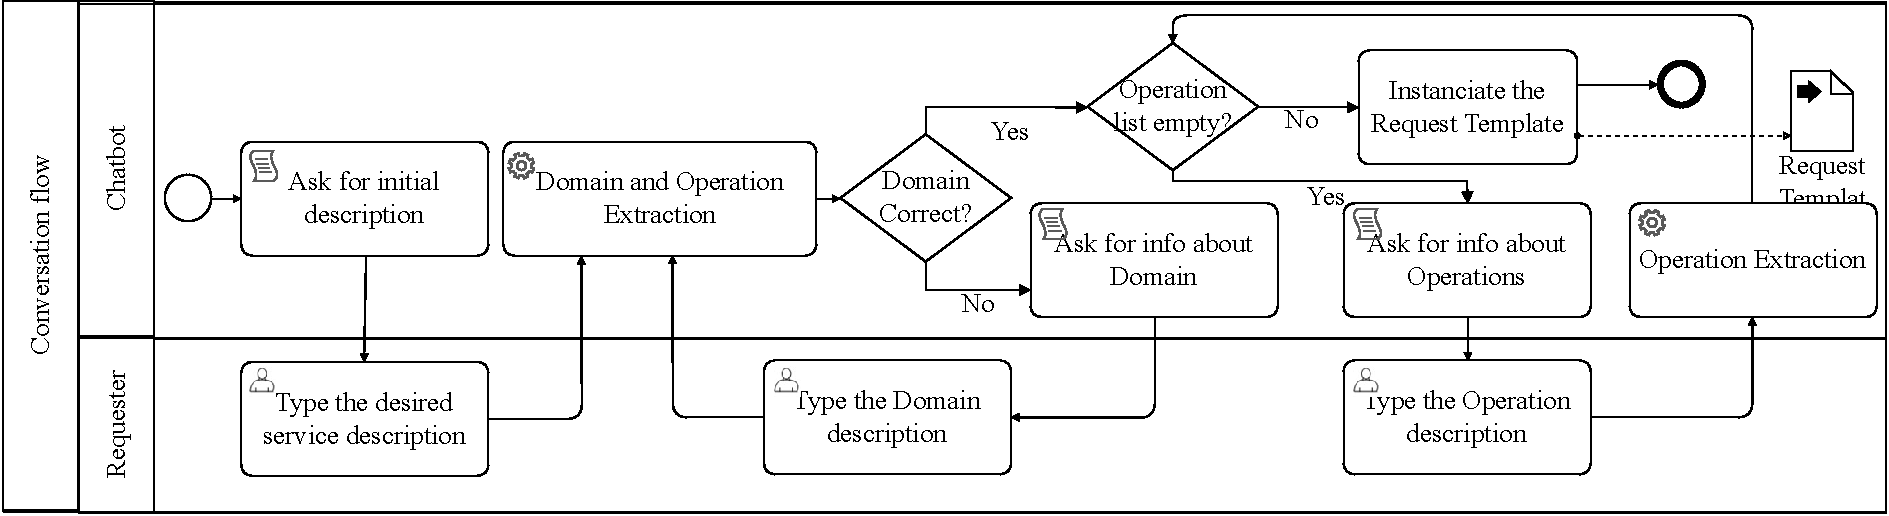
\includegraphics[width=0.85\textwidth]{../figures/MyFigures/ConversationFlow.drawio.pdf}
\captionsetup{justification=centering}
\caption{\gls{disco} Conversation Flow}\label{fig:disco-flow}
}
\end{figure}

\vspace{-10pt}
\hypertarget{sec:Component-retrieval-engine}{%
\subsection{Component Retrieval Engine}\label{sec:Component-retrieval-engine}}
\vspace{10pt} 	

Following the parameter identification, the subsequent step involves retrieving the appropriate component accordingly. The Component Retrieval Engine is tasked with matching a component’s metadata to the desired operations specified in a query. The metadata was created during the component generation phase described in \cref{sec:component-gen} by applying the query expansion techniques on the \gls{api} textual description. The figure below illustrates the detailed process of extracting these operations:

\begin{figure}[hbt]
\hypertarget{fig:disco-retrieve}{%
\centering
\includegraphics[width=0.85\textwidth]{../figures/MyFigures/retrival.pdf}
\captionsetup{justification=centering}
\caption{Component Retrieval Procedure}\label{fig:disco-retrieve}
}
\end{figure}


\vspace{-10pt}
\hypertarget{sec:solution-Designer}{%
\section{Solution Designer}\label{sec:solution-Designer}}
\vspace{10pt}

Once the best components are found, next step involves finding the possible compatibility paths among them based on the query. In cases where the domain expert's goal cannot be fulfilled by deploying a singular component, a composite solution becomes necessary. Finding a compatible sequence of components capable of collectively addressing the domain expert's query is defined as composition problem: 
\begin{thesisdefinition}{Composition Problem}{def:composition-problem}
For each query \(Q\), the composition problem is defined as
\(< Q.I,\ Q.O >\), where \(Q.I\) and \(Q.O\) represent the query's input
and output respectively and a list of components denoted as\(\  < c_{1},\ldots,\ c_{n} >\), the composition problem is concerned
with automatically generating a Directed Acyclic Graph (DAG) of
components that satisfies the following conditions:
\begin{itemize}
\item
  \(\exists\ c_{i} \in \left\{ c_{1},\ \ldots,\ c_{n} \right\}\ |\ c_{i}.I \subseteq Q.I\).
At least one component has inputs that are a subset of the
query\textquotesingle s inputs.
\item 
\(\exists\ c_{j} \in \left\{ c_{1},\ \ldots,\ c_{n} \right\}|\ c_{j}.O \supseteq Q.O\).
At least one component has outputs that are a superset of the
query\textquotesingle s outputs.

\item
  \(\forall\ c_{i}\ ,\ c_{j\ }|c_{i}.O \subseteq c_{j}.I\  \cup \ c_{i}.I\  \supseteq c_{j}.O\mathbf{\ }\).
  A path exists between components \(c_{i}\) and \(c_{j}\) such that the
  output of \(c_{i}\)\hspace{0pt} is a subset of or compatible with the
  input of \(c_{j}\)\hspace{0pt}, and the input of \(c_{i}\ \)includes
  or overlaps with the output of \(c_{j}\)
\end{itemize}
\end{thesisdefinition}

In this context, \(c_{i}.I\) and \(c_{i}.I\) represent the inputs of the
component \(c_{i}\) and \(c_{j}\)\hspace{0pt}, respectively, while
\(c_{i}.O\) and \(c_{j}.O\) represent their outputs. The goal is to
construct a \gls{dag} that maps the flow from the query's
input to its output through the available component, satisfying the
specified inclusion relationships.

According to \autocite{Lee2013}, two components are considered composable if
the output parameter of one component can be consumed as the input
parameter for another. Consequently, the composition problem involves
searching the compatibility graph with the initial
query's input serving as the starting node. If each
involved component has only one input and one output, the problem
exhibits linear complexity. However, if components have multiple inputs
or outputs, the problem's complexity becomes exponential
\autocite{Serrano2020, Lee2013}.

\begin{figure}[hbt]
\hypertarget{fig:disco-sd}{%
\centering
\includegraphics[width=0.85\textwidth]{../figures/MyFigures/SolutionDesignerBPMN.drawio.pdf}
\captionsetup{justification=centering}
\caption{Solution Designing \gls{bpmn} Process Diagram}\label{fig:disco-sd}
}
\end{figure}

The Solution Designer addresses the composition problem by generating a compatibility graph based on the query and candidate components. This graph dictates the intercomponent communication flow. The \gls{bpmn} diagram in \cref{fig:disco-sd}shows the steps for this process.


\vspace{-15pt}
\hypertarget{sec:graph-gen}{%
\subsection{Compatibility Graph Generation}\label{sec:graph-gen}}
\vspace{10pt}

The compatibility graph represents the potential paths between the selected components. The compatibility Graph is formally defined as:

\begin{thesisdefinition}{Compatibility Graph}{def:compatobility-gaph}
The compatibility graph denoted as
\(CG = (V,\ E)\), is a directed acyclic graph defined as follows:
\begin{itemize}
\item
\(V = \{ v|v = (id,s)\}\) represents the vertex set where each vertex
  \(v\) represents a component and has a unique identifier \(id\). The
  state, \(s\) indicates the status of each component, which can be
  "Blocked" in the case of isolated components. The vertices \(a_{o\ }\)
  and \(a_{f}\) represent the starting and final points of the solution,
  respectively.
\item 
\(E = \{ e|e = (c_{i},\ c_{j},t)\}\ \)is the edge set, where each edge
  \(e\) represents a possible communication between two components
  \(c_{i}\) and \(c_{j}\)\hspace{0pt}, with \(t\) providing a textual
  annotation of this communication.
 
\end{itemize}
\end{thesisdefinition}

In the initial phase, the Solution Designer constructs a weighted
compatibility graph by employing Algorithm 6.3.
This algorithm begins with an empty graph, incrementally adding vertices
for each component within the set E. All Components are mapped to a
vertex and the edge \(e_{ij}\) is established if input of \(c_{i}\) can
be consumed by \(c_{j}\) as determined by the similarity score. The
similarity score, which ranges from 1 to 3, dictates the weight of each
edge, with 3 indicating the strongest connection between the components.

\setlength{\algomargin}{2em} %
\begin{algorithm}
	\DontPrintSemicolon
	\KwIn{Finite set C\(= \{ c_{1},\ \ldots,\ c_{n}\}\) of
	components}
	\KwOut{Compatibility Graph \(CG = (V,\ E)\)}
	
	\begin{enumerate}
	\item 
	Initialize \(\mathbf{V = \ }\mathbf{\varnothing\ }\)and
	  \(\mathbf{E = \ \varnothing}\)
	\item 
		\ForEach{component \(\mathbf{c}_{\mathbf{i}}\mathbf{\  \in C}\)}
			{
			\begin{enumerate}
							  \def\labelenumii{\alph{enumii}.}
							  \item
							  Add a new vertex \(\mathbf{v}_{\mathbf{i}}\) corresponding
							    to\(\mathbf{c}_{\mathbf{i}}\) in \(\mathbf{V}\).
							  \end{enumerate}
			}\label{endfor}
	\item 
	\ForEach{pair of components
	  \(\left( \mathbf{c}_{\mathbf{i}}\mathbf{,\ }\mathbf{c}_{\mathbf{j}} \right)\mathbf{:}\)}
				{
				\begin{enumerate}
								  \def\labelenumii{\alph{enumii}.}
								  \item
								    Initialize \(\mathbf{weight}\mathbf{\ }\mathbf{=}\mathbf{0}\).
								  \item
								 		If
								   \(\mathbf{c}_{\mathbf{i}}\mathbf{.}\mathbf{O}\mathbf{.}\mathbf{dataType}\mathbf{=}\mathbf{c}_{\mathbf{j}}\mathbf{.}\mathbf{I}\mathbf{.}\mathbf{dataType}\)
								   and
								   \(\mathbf{c}_{\mathbf{i}}\mathbf{.}\mathbf{O}\mathbf{=}\mathbf{c}_{\mathbf{j}}\mathbf{.}\mathbf{I}\),
								   then
								   \(\mathbf{weight}\mathbf{\ }\mathbf{=}\mathbf{weight}\mathbf{+ 3}\).
								   
								   \item 
								   If
								     \(semanticSim\left( s_{i}.O.param,\ s_{j}.I.Param \right) > similarity\_ threshold,\ \)then
								     \(weight\  = weight + 2\).
								     \item 
								     If
								       \(semanticSim\left( s_{i}.O.desc,\ s_{j}.I.desc \right) > similarity\_ threshold\),
								       then \(weight\  = weight + 1\).
								  \end{enumerate}
				}\label{endfor}
	
	\item 
	If \(\mathbf{weight}\mathbf{> 0}\), then add edge
	  \(\mathbf{e}_{\mathbf{ij}}\) with \(\mathbf{weight}\) to
	  \(\mathbf{E}\)
	  \item 
	  Return the
	    \(\mathbf{CG}\mathbf{= (}\mathbf{V}\mathbf{,\ }\mathbf{E}\mathbf{)}\).
	\end{enumerate}
	
\caption{Compatibility Graph Generation}\label{alg:disc-cg}
\end{algorithm}

The algorithm evaluates the compatibility between \(c_{i}\) and
\(\ c_{j}\) using a three-tiered approach involving both syntactic and
semantic comparisons. At the first level, the syntactic compatibility is
determined by comparing the output and input attributes of
\(c_{i}\ \)and \(c_{j}\). If both the name and data type match, the edge
\(e_{ij}\) is assigned with the highest weight of 3. Following this
direct syntactic match, the algorithm calculates the parameter semantic
similarity between input and output parameters of \(c_{i}\ \)and
\(c_{j}\) using \gls{nlp} techniques. A match at this level adds up the edge
weight by 2. As last level, the algorithm calculates the similarity of
the textual descriptions of the inputs and outputs. this condition
contributes 1 to the edge weight. The highest compatibility score is
achieved when components are composable at both syntactic and semantic
levels, ensuring a comprehensive assessment of their interoperability.

\cref{fig:disco-cg-test} shows an example of compatibility graph for candidate
components identified in response to the query: "Find the weather
temperature and location based on the IP or telephone number." The
query input parameter is identified as \(Q.I = \{ IP,\ Tel\ number\}\)
which is the starting point for graph traversal and
\(Q.O = \{ Temprature,\ Location\}\) should be the output parameter of
the final component.

\begin{figure}[hbt]
\hypertarget{fig:disco-cg-test}{%
\centering
\includegraphics[width=0.85\textwidth]{../figures/MyFigures/test1.png}
\captionsetup{justification=centering}
\caption{Compatibility Graph for an example Query}\label{fig:disco-cg-test}
}
\end{figure}

Compatibility graph can produce several composition paths, some of which may be non-relevant or redundant. The composition must generate all of the query’s output parameters by utilizing all or part of the input parameters. The purpose of composition path refinement, depicted in \cref{fig:disco-sd}, is to limit the number of potential composition chains according to the following rules:

\begin{itemize}
\item
  \(c_{o} \subseteq Q.I\) and \(c_{f} \supseteq Q.O\) denotes that the
  initial component accepts the query's input and the final component
  \(c_{f}\) produces the query's output.
\item
  The chains with the minimum number of components should be
  prioritized. This rule ensures the lowest cost for data transfer among
  the components.
\item
  Duplicated chains are eliminated. This rule filters out the chains
  that are permutated of previous processed chains.
\end{itemize}

To address the example query, the subsequent chains have been identified. Following the third rule stated above, the first chain is eliminated to prevent redundancy.

\[< IPToLocation,WeatherAPI >\]
\[\  < IPToLocation,WeatherAPI,\ GeoLocationTime >\]
\[< NumberToAreaCode,\ WeatherAPI >\]

After refining the valid paths, it is necessary to rank then to identify
the most efficient option. The ranking score is determined by evaluating
the similarity between the components' input, output, and description,
represented as the edge\textquotesingle s weight. The following table
shows the list of ranked composition paths:

\hypertarget{tbl:disco-composition-paths}{}
\begin{longtable}{@{}ccp{0.65\linewidth}@{}}
\caption{\label{tbl:disco-composition-paths}The Ranked List of Composition Paths}\tabularnewline
\toprule
\textbf{Rank} & \textbf{Score} & \textbf{Composition Path} \tabularnewline
\midrule
\endfirsthead

\toprule
\textbf{Rank} & \textbf{Score} & \textbf{Composition Path} \tabularnewline
\midrule
\endhead

1 & 5 & \(< \text{IPToLocation}, \text{WeatherAPI}, \text{GeoLocationTime} >\) \tabularnewline
2 & 3 & \(< \text{IPToLocation}, \text{WeatherAPI} >\) \tabularnewline
3 & 2 & \(< \text{NumberToAreaCode}, \text{WeatherAPI} >\) \tabularnewline

\bottomrule
\end{longtable}

The composition path that receives the highest score, is considered as the final compatibility graph. This graph is then incorporated into the composition model, following the definition provided in \cref{sec:solution}.

\vspace{-10pt}
\hypertarget{sec:disco-evaluation}{%
\section{Evaluation}\label{sec:disco-evaluation}}
\vspace{10pt}
This section presented the evaluation process of \gls{disco} and Solution
Designer tools to address the limited expressive power subproblem and
achieve \cref{ro:2}. According to the requirements outlined in \cref{sec:requirements}, \gls{disco} and Solution Designer should fulfill the Semi-Automation and
Functionality Integration requirements at the development process level,
and the Effectiveness at the tool's level.

\gls{disco} fully satisfies the \emph{Semi-Automation} requirement. The
discovery process is entirely automated, yet it allows domain expert to
review and refine the final list of candidate components. The solution
Designer, on the other hand, performs fully automated without the domain
expert's intervention. Therefore, it partially satisfies this
requirement.

The \emph{Functionality Integration} is fully satisfied by both DisCo
and Solution Designer. These tools provide structured process for
component discovery and composition paths generation. New components can
be integrated into the composition if they satisfy the composition
rules.

Comprehensive evaluations of each tool, in terms of effectiveness are
provided in the following two sections.

\vspace{-10pt}
\hypertarget{sec:disco-evaluation-disco}{%
\subsection{\gls{disco} Evaluation}\label{sec:disco-evaluation-disco}}

To further evaluate the performance of DisCo, a series of experiments were conducted within the context of a user study. The step-by-step process is outlined below:

\textbf{Pre-processing and dataset design}
The initial step involves preparing the dataset. For this purpose, we
used ProgrammableWeb (PW) and Guru\footnote{\url{https://apis.guru/}},
two public service registries, as our sources for \gls{api} data. Descriptive
data for 500 web \gls{api}s, including their names, descriptions, and
categories, were collected. These \gls{api}s were randomly selected from the
five most popular domains on PW. According to PW, popularity is
determined by the proportion of mashups that rely on the \gls{api}s within a
particular domain\footnote{\url{https://www.programmableweb.com/faq}}.
The proportion of \gls{api}s in each category was calculated as the ratio of
\gls{api} in that domain to the total number of registered \gls{api}s across all
selected domains. The following diagram illustrates the distribution of
\gls{api}s in our registry: 

\begin{figure}[hbt]
\hypertarget{fig:disco-evaluation-result}{%
\centering
\includegraphics[width=0.85\textwidth]{../figures/MyFigures/APIStat.pdf}
\captionsetup{justification=centering}
\caption{Operations Extracted from RadMap API}\label{fig:disco-APIStat}
}
\end{figure}


The descriptive data of each \gls{api} was processed to extract the operations as described in \cref{sec:disco}. An example of extracted \gls{api} operations is shown in the following figure:

\begin{figure}[hbt]
\hypertarget{fig:disco-evaluation-result}{%
\centering
\includegraphics[width=0.85\textwidth]{../figures/MyFigures/radmap.png}
\captionsetup{justification=centering}
\caption{Operations Extracted from RadMap API}\label{fig:disco-evaluation-result}
}
\end{figure}

\textbf{Experiment design and procedure}
For the user study, we recruited 15 participants, including undergraduate and postgraduate students as well developers, to assess the usability of the \gls{disco}. The experiment runs on a local platform instance. The details of the recruitment process and evaluation task list are presented Appendix.
To evaluate \gls{disco}, each participant was assigned to a specific domain and tasked with constructing three queries within that domain, without any length restriction. In total, 45 queries were constructed and for each, \gls{disco} engaged in multiple rounds of conversation with the users to identify the target domain and the desired operations.  \cref{fig:disco-conversation} presents examples of these conversations and display the ranked components according to their similarity scores.

\begin{figure}[hbt]
\hypertarget{fig:disco-conversation}{%
\centering
\includegraphics[width=0.85\textwidth]{../figures/MyFigures/DosCoCon.png}
\captionsetup{justification=centering}
\caption{Example Conversation Round with DisCo}\label{fig:disco-conversation}
}
\end{figure}

\textbf{Result}

The retrieved components were evaluated by participants using a rating
scale from 0 to 3. A rating of ``0'' indicates irrelevant components
with meaningless operations. A rating of ``1'' is assigned to components
that are poorly relevant and lack specificity to match the participant's
intention. Ratings of "2" and "3" denote relevant and highly
relevant operations with identified parameters, respectively.

An analysis of 45 queries revealed that the domain identification
process achieved a success rate of 91\%. The ranking of the retrieved
components for each query is presented in \cref{tbl:disco-eval}. The precision of
our approach in retrieving suitable components is 0.78 and the recall
value is computed as 0.80.

\hypertarget{tbl:disco-eval}{}
\begin{longtable}{@{}llll@{}}
\caption{\label{tbl:disco-eval}\gls{disco} Evaluation Result}\tabularnewline
\toprule
\begin{minipage}[b]{0.23\columnwidth}\raggedright
Irrelevant\strut
\end{minipage} & 
\begin{minipage}[b]{0.24\columnwidth}\raggedright
Poorly Relevant\strut
\end{minipage} & 
\begin{minipage}[b]{0.24\columnwidth}\raggedright
Relevant\strut
\end{minipage} & 
\begin{minipage}[b]{0.29\columnwidth}\raggedright
Highly Relevant\strut
\end{minipage} \tabularnewline
\midrule
\endfirsthead

\toprule
\begin{minipage}[b]{0.23\columnwidth}\raggedright
Irrelevant\strut
\end{minipage} & 
\begin{minipage}[b]{0.24\columnwidth}\raggedright
Poorly Relevant\strut
\end{minipage} & 
\begin{minipage}[b]{0.24\columnwidth}\raggedright
Relevant\strut
\end{minipage} & 
\begin{minipage}[b]{0.29\columnwidth}\raggedright
Highly Relevant\strut
\end{minipage} \tabularnewline
\midrule
\endhead

10\% & 10\% & 20\% & 60\% \tabularnewline

\bottomrule
\end{longtable}

\vspace{-10pt}
\hypertarget{sec:eval-sd}{%
\subsection{Solution Designer Evaluation}\label{sec:eval-sd}}
\vspace{10pt}

The Solution Designer performance is evaluated by measuring precision
and recall. Precision measures accuracy by calculating the number of
relevant compositions generated, while recall assesses the coverage of
the generated solutions.

To measure these metrics, 15 components from diverse domains were
selected, ensuring comprehensive coverage of various scenarios. Although
rea-world scenarios are typically restricted to particular domain,
including diverse components enhances the reliability of the evaluation.
The algorithm\textquotesingle s performance is assessed under three
different similarity threshold settings for \(semanticSim\): 0.55, 0.6
and 0.65. For each setting, a compatibility graph is generated, as
illustrated in \cref{fig:eval-sd-test}.

\begin{figure}[hbt]
\hypertarget{fig:eval-sd-test}{%
\centering
\includegraphics[width=0.85\textwidth]{../figures/MyFigures/Compatibility graph.pdf}
\captionsetup{justification=centering}
\caption{Compatibility Graphs with Different Similarity Threshold. a)semanticSim = 0.55 b)semanticSim =0.6}\label{fig:eval-sd-test}
}
\end{figure}
\pagebreak
The precision and recall are calculated according to these formulas:

\(precision\  = \ \frac{tp}{tp + fp}\)
\(recall\  = \ \frac{tp}{tp + fn}\)

where \(tp\) (True Positives) represents the number of correctly
identified composition paths, \(tn\) (True Negatives) denotes the number
of components that have not been composed correctly, \(fp\) (False
Positives) is the number of components that were mistakenly identified
as composable and \(fn\) (False Negatives) are the composition paths
that were missed.

The precision and recall for each compatibility graph is presented in
Table below:

\hypertarget{tbl:sd-result}{}
\begin{longtable}{@{}llll@{}}
\caption{\label{tbl:sd-result}Solution Designer Evaluation Result}\tabularnewline
\toprule

SemanticSim &  &  & Precision / Recall \tabularnewline
\midrule
\endfirsthead

\toprule
SemanticSim &  &  & Precision / Recall \tabularnewline
\midrule
\endhead

\bottomrule
\endlastfoot

0.55 & TP = 12 & FP = 10 & Precision = 0.54 \tabularnewline
 & FN = 3 & TN = 147 & Recall = 0.8 \tabularnewline
 & \multicolumn{3}{l}{Total = 22} \tabularnewline
\midrule

0.6 &TP = 12 & FP = 0 & Precision = 1 \tabularnewline
 & FN = 3 & TN = 157 & Recall = 0.8 \tabularnewline
 & \multicolumn{3}{l}{Total = 12} \tabularnewline
\midrule

0.65 & TP = 8 & FP = 0 & Precision = 1 \tabularnewline
 & FN = 7 & TN = 161 & Recall = 0.53 \tabularnewline
 & \multicolumn{3}{l}{Total = 8} \tabularnewline
\end{longtable}
\vspace{-15pt}

The efficiency of the Algorithm \hyperref[Algorithm63]{6.3} is evaluated
based on its algorithmic complexity. The algorithm operates on a finite
set of \(n\) components, executing two nested loops, resulting in a
total of \(n^{2}\) iterations. Within the inner loop, compatibility
comparisons performed, each with a time complexity of \(O(1)\).
Consequently, the overall time complexity of the algorithm is
\(O(n^{2})\), which is acceptable.

\pagebreak
\vspace{-15pt}
\hypertarget{sec:disc.summary}{%
\section{Summary}\label{sec:disc.summary}}
\vspace{10pt}

This chapter introduced two mechanisms designed to support domain experts during the component discovery and composition design phases. These mechanisms aim to enhance the situational application’s expressive power by offering a natural-language-based interaction medium (\gls{disco}) for component discovery purposes. Moreover, by defining suitable composition choreography, Solution Designer enhances the expressiveness by generating the most efficient solution class. The individual evaluation of each mechanism is detailed in \cref{sec:disco-evaluation}. The overall performance of these mechanisms, as integrated within the \gls{dsac}, is assessed in Chapter 7.